\documentclass{article}
\usepackage[margin=1in]{geometry}
%\documentclass[]{aiaa-tc}% insert '[draft]' option to show overfull boxes
\usepackage[utf8]{inputenc}
\usepackage{amsmath}
\usepackage{float}
\usepackage{graphicx} % needed for figures

\title{MEEN 534 Term Project}
\author{Dustan Kraus and Erich Mielke}
\date{April 2017}

\begin{document}

\maketitle

\section{Introduction}
The objective of this project was to model the attitude dynamics of the Apollo Command Service Module spacecraft. The following sections contain the results we found from each task of this project.

\section{Task A: Inertial Properties}
\subsection{Part (a): General Case}
\subsubsection{Part (a): Location of center of mass}
The location of the center of mass of the combined command and service modules (CSM) including propellant, relative to the A frame and expressed in the A frame (which is equivelant to being expressed in the B frame at the center of mass) is $\mathbf{P_{cm} = 23.6177\hat{i} + 0.0961\hat{j} - 0.0087\hat{k}}$ \textbf{meters}.

\subsubsection{Part (b): Inertia Matrix}
The total inertia matrix of the CSM, including propellant, about the body-fixed B axes at the center of mass of the CSM is: 

\[
%\begin{equation}
I_B=
  \begin{bmatrix}
    40822.99 & 1537.28 & -3178.21 \\
    1537.28 & 90578.41 & 128.53 \\
    -3178.21 & 128.53 & 98727.82
  \end{bmatrix} \:\text{kg-$m^2$}
%\end{equation}
\]

\subsection{Part (b): Simplified Case}
This section includes the same calculations as above for the center of mass and the inertia matrix, except, the centers of mass of all components are located on the x axis.

\subsubsection{Part (a): Location of center of mass}
The location of the CSM including propellant and relative to the A frame and expressed in the A frame (which is equivelant to being expressed in the B frame at the center of mass) is $\mathbf{P_{cm} = 23.6177\hat{i} + 0\hat{j} + 0\hat{k}}$ \textbf{meters}.

\subsubsection{Part (b): Inertia Matrix}
The total inertia matrix of the CSM, including propellant, about the body-fixed B axes at the center of mass of the CSM is: 

\[
I_B=
  \begin{bmatrix}
    40482.01 & 0 & 0 \\
    0 & 90343.32 & 0 \\
    0 & 0 & 98621.94
  \end{bmatrix} \:\text{kg-$m^2$}
\]

\section{Task B: Equations of Motion}
This task was to find the rotational equations of motion that could be solved numerically to find the orientation of the spacecraft ($\psi, \theta, \phi$) given torque inputs about the body-fixed (B frame) xyz axes. The six 1st-order equations are shown below in Eqs~\ref{eq:M} - \ref{eq:euler_dot}.

\begin{equation}\label{eq:M}
%\begin{aligned}
M=
  \begin{bmatrix}
    Ixx & -Ixy & -Ixz \\
    -Ixy & Iyy & -Iyz \\
    -Ixz & -Iyz & Izz
  \end{bmatrix}
%\end{aligned}
\end{equation}
\begin{equation}
F = 
  \begin{bmatrix}
  -I_{xy} \omega_x \omega_z + I_{xz} \omega_x \omega_y + (I_{yy} - I_{zz}) \omega_y \omega_z + I_{yz} (\omega_y^2 - \omega_z^2) + M_x \\
  -I_{yz} \omega_x \omega_y + I_{xy} \omega_y \omega_z + (I_{zz} - I_{xx}) \omega_x \omega_z + I_{xz} (\omega_z^2 - \omega_x^2) + M_y \\
  -I_{xz} \omega_y \omega_z + I_{yz} \omega_x \omega_z + (I_{xx} - I_{yy}) \omega_x \omega_y + I_{xy} (\omega_x^2 - \omega_y^2) + M_z
  \end{bmatrix}
\end{equation}

\begin{equation}
\begin{bmatrix}
\dot{\omega_x} \\
\dot{\omega_y} \\
\dot{\omega_z}
\end{bmatrix}=
M^{-1}F
\end{equation}
\begin{equation}\label{eq:euler_dot}
\begin{bmatrix}
\dot{\psi} \\
\dot{\theta} \\
\dot{\phi}
\end{bmatrix}=
\begin{bmatrix}
\dfrac{1}{cos(\theta)}(\omega_y sin(\phi) + \omega_z cos(\phi)) \\
%1/cos(\theta) \\
\omega_y cos(\phi) - \omega_z sin(\phi) \\
\dfrac{1}{cos(\theta)} (\omega_y sin(\theta) sin(\phi) + \omega_z sin(\theta) cos(\phi)) + \omega_x
\end{bmatrix}
\end{equation}

\section{Task C: Simulations and Calculations}
\subsection{Part (a): Matlab Function}
We created and submitted a matlab function called \verb|mielke_kraus.m| that simulates the rotational motion of the CSM in response to applied torques.

\subsection{Part (b): Simulated Response to Applied Torques}
We simulated and plotted the response to the following torque inputs for both the general and simplified case (see Figures~\ref{fig:gen_case} and \ref{fig:sim_case}).

\begin{equation}\label{eq:Mx_app}
M_x(t) = 176 cos(0.2 t)  \:\text{N-m}
\end{equation}
\begin{equation}
M_y(t) = 54  \:\text{N-m}
\end{equation}
\begin{equation}\label{eq:Mz_app}
M_z(t) = 98 sin(0.3 t)  \:\text{N-m}
\end{equation}

Table~\ref{tab:max_min} on page~\pageref{tab:max_min} includes the maximum and minimum values for both cases.

\begin{figure}[H]
  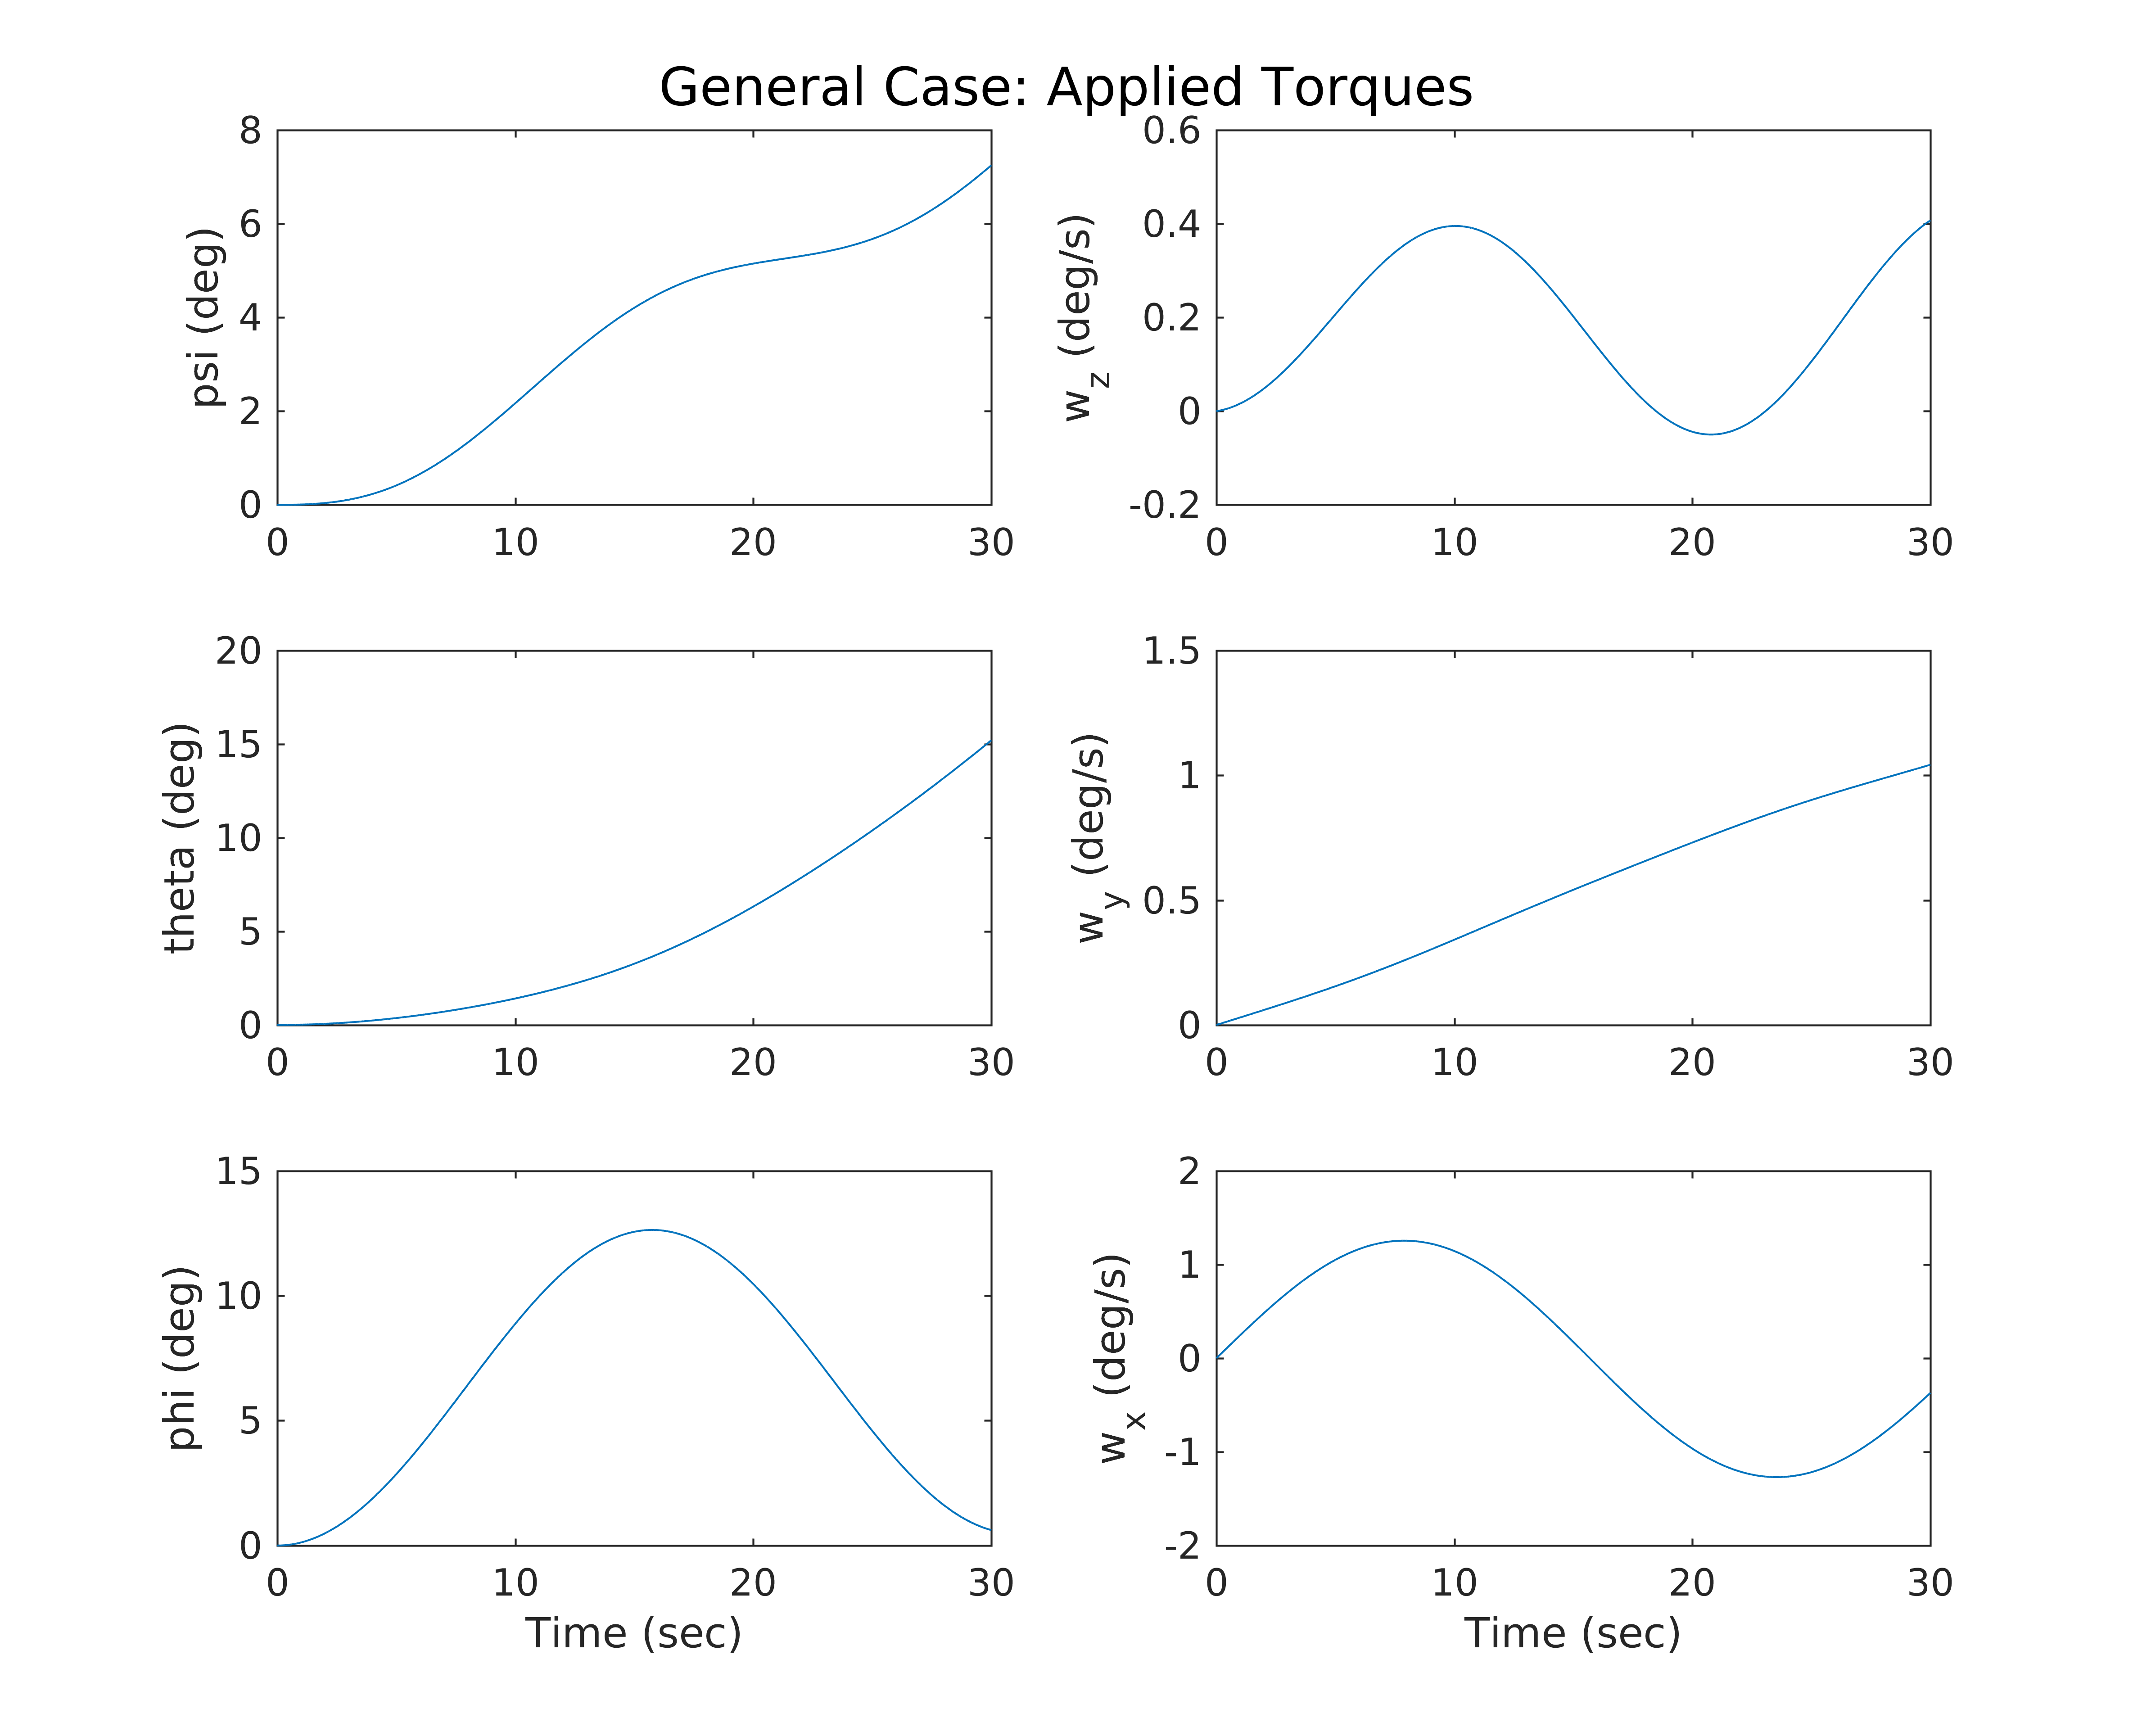
\includegraphics[width=\linewidth]{general_case.png}
  \caption{This figure contains the simulated response to the applied torque inputs in Eqs.~\ref{eq:Mx_app} - \ref{eq:Mz_app} for the general case.}
  \label{fig:gen_case}
\end{figure}

\begin{figure}[H]
  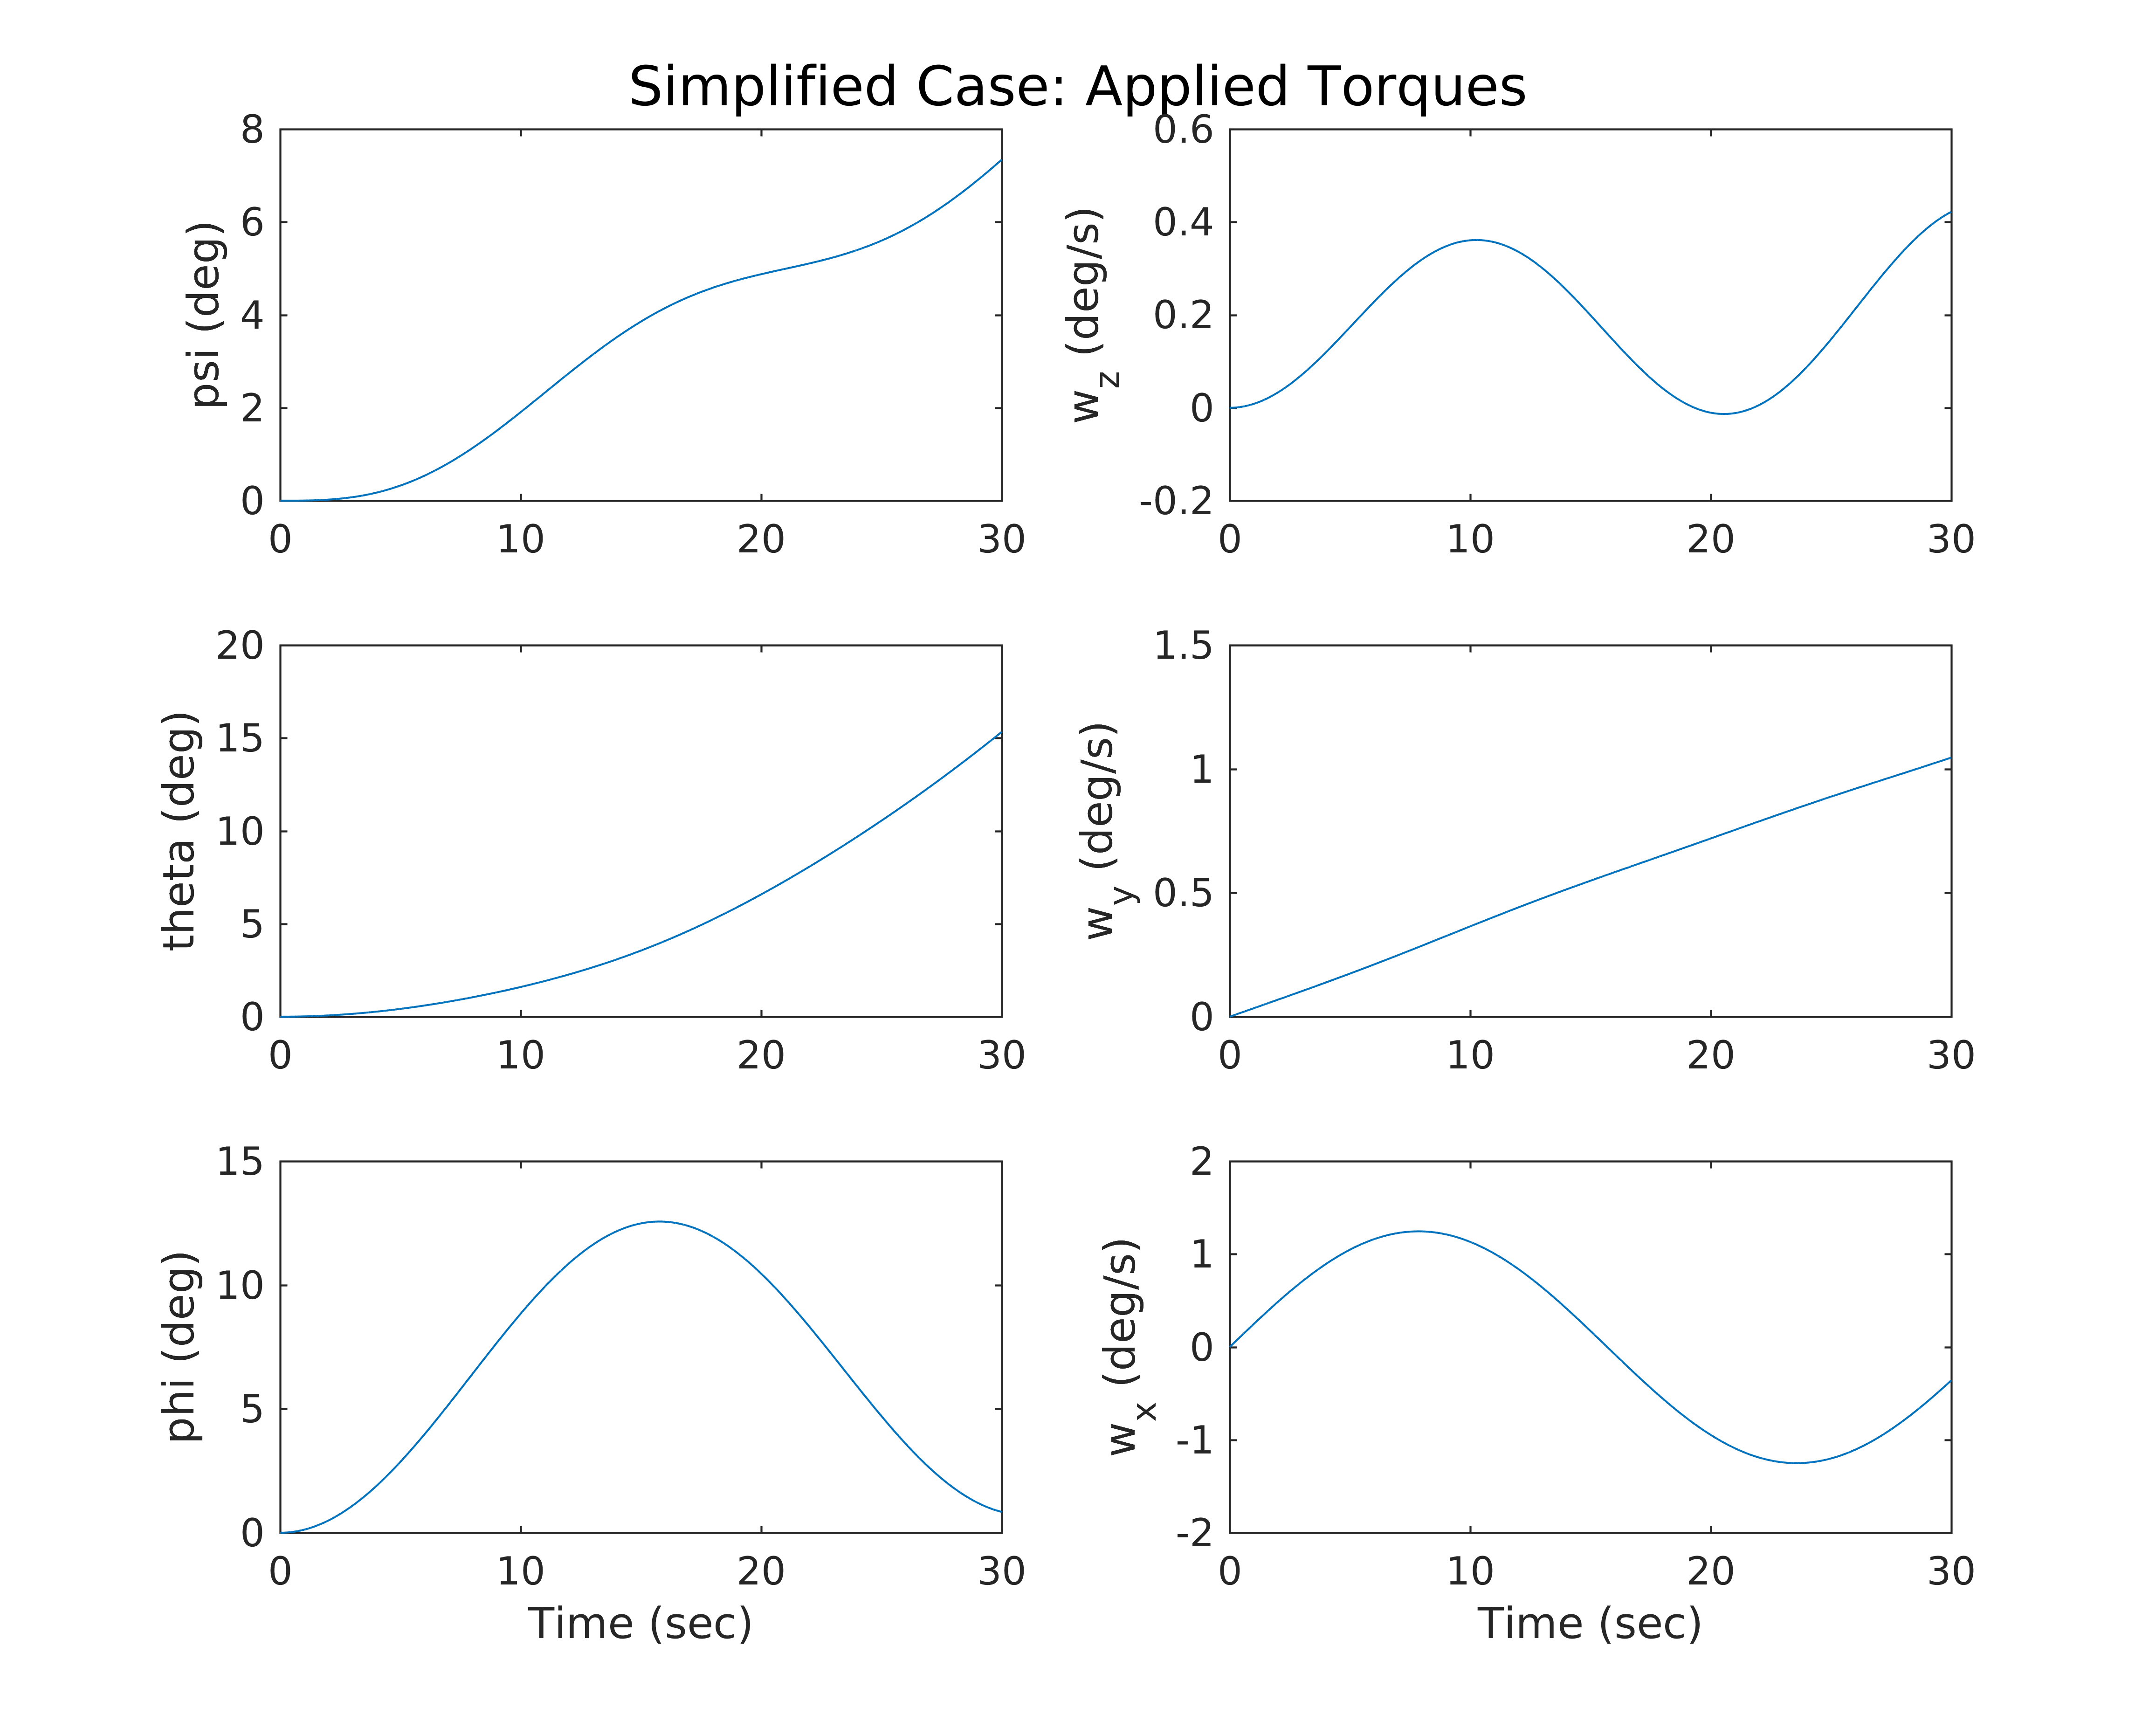
\includegraphics[width=\linewidth]{simplified_case.png}
  \caption{This figure contains the simulated response to the applied torque inputs in Eqs.~\ref{eq:Mx_app} - \ref{eq:Mz_app} for the simplified case.}
  \label{fig:sim_case}
\end{figure}

\subsection{Part (c): Barbeque Mode}\label{BBQ}
During the flight to the moon, the CSM was placed in passive thermal control mode (barbeque mode), in which the CSM rotated at a constant rate about the x axis to maintain even heating and cooling. We found the required torque values to maintain a constant x-axis rotation of 1 deg/s without motion about the other axes (using the general case inertia matrix).
\[
\begin{bmatrix}
M_x \\
M_y \\
M_z
\end{bmatrix}=
\begin{bmatrix}
0 \\
0.9681 \\
0.4683
\end{bmatrix} \:\text{N-m}
\]

We then simulated barbeque mode by assigning an initial condition of 1 deg/s for $\omega_x$ and zero initial conditions for the other states. Figure~\ref{fig:calc_torque} shows the response of the system with the calculated torques applied. As shown, the system rotates about only the x axis. Figure~\ref{fig:zero_torque} shows the response of the system with zero torque inputs applied in barbeque mode. Without the calculated torques applied, the system develops angular velocity about the y and z axes as well.

\begin{figure}[H]
  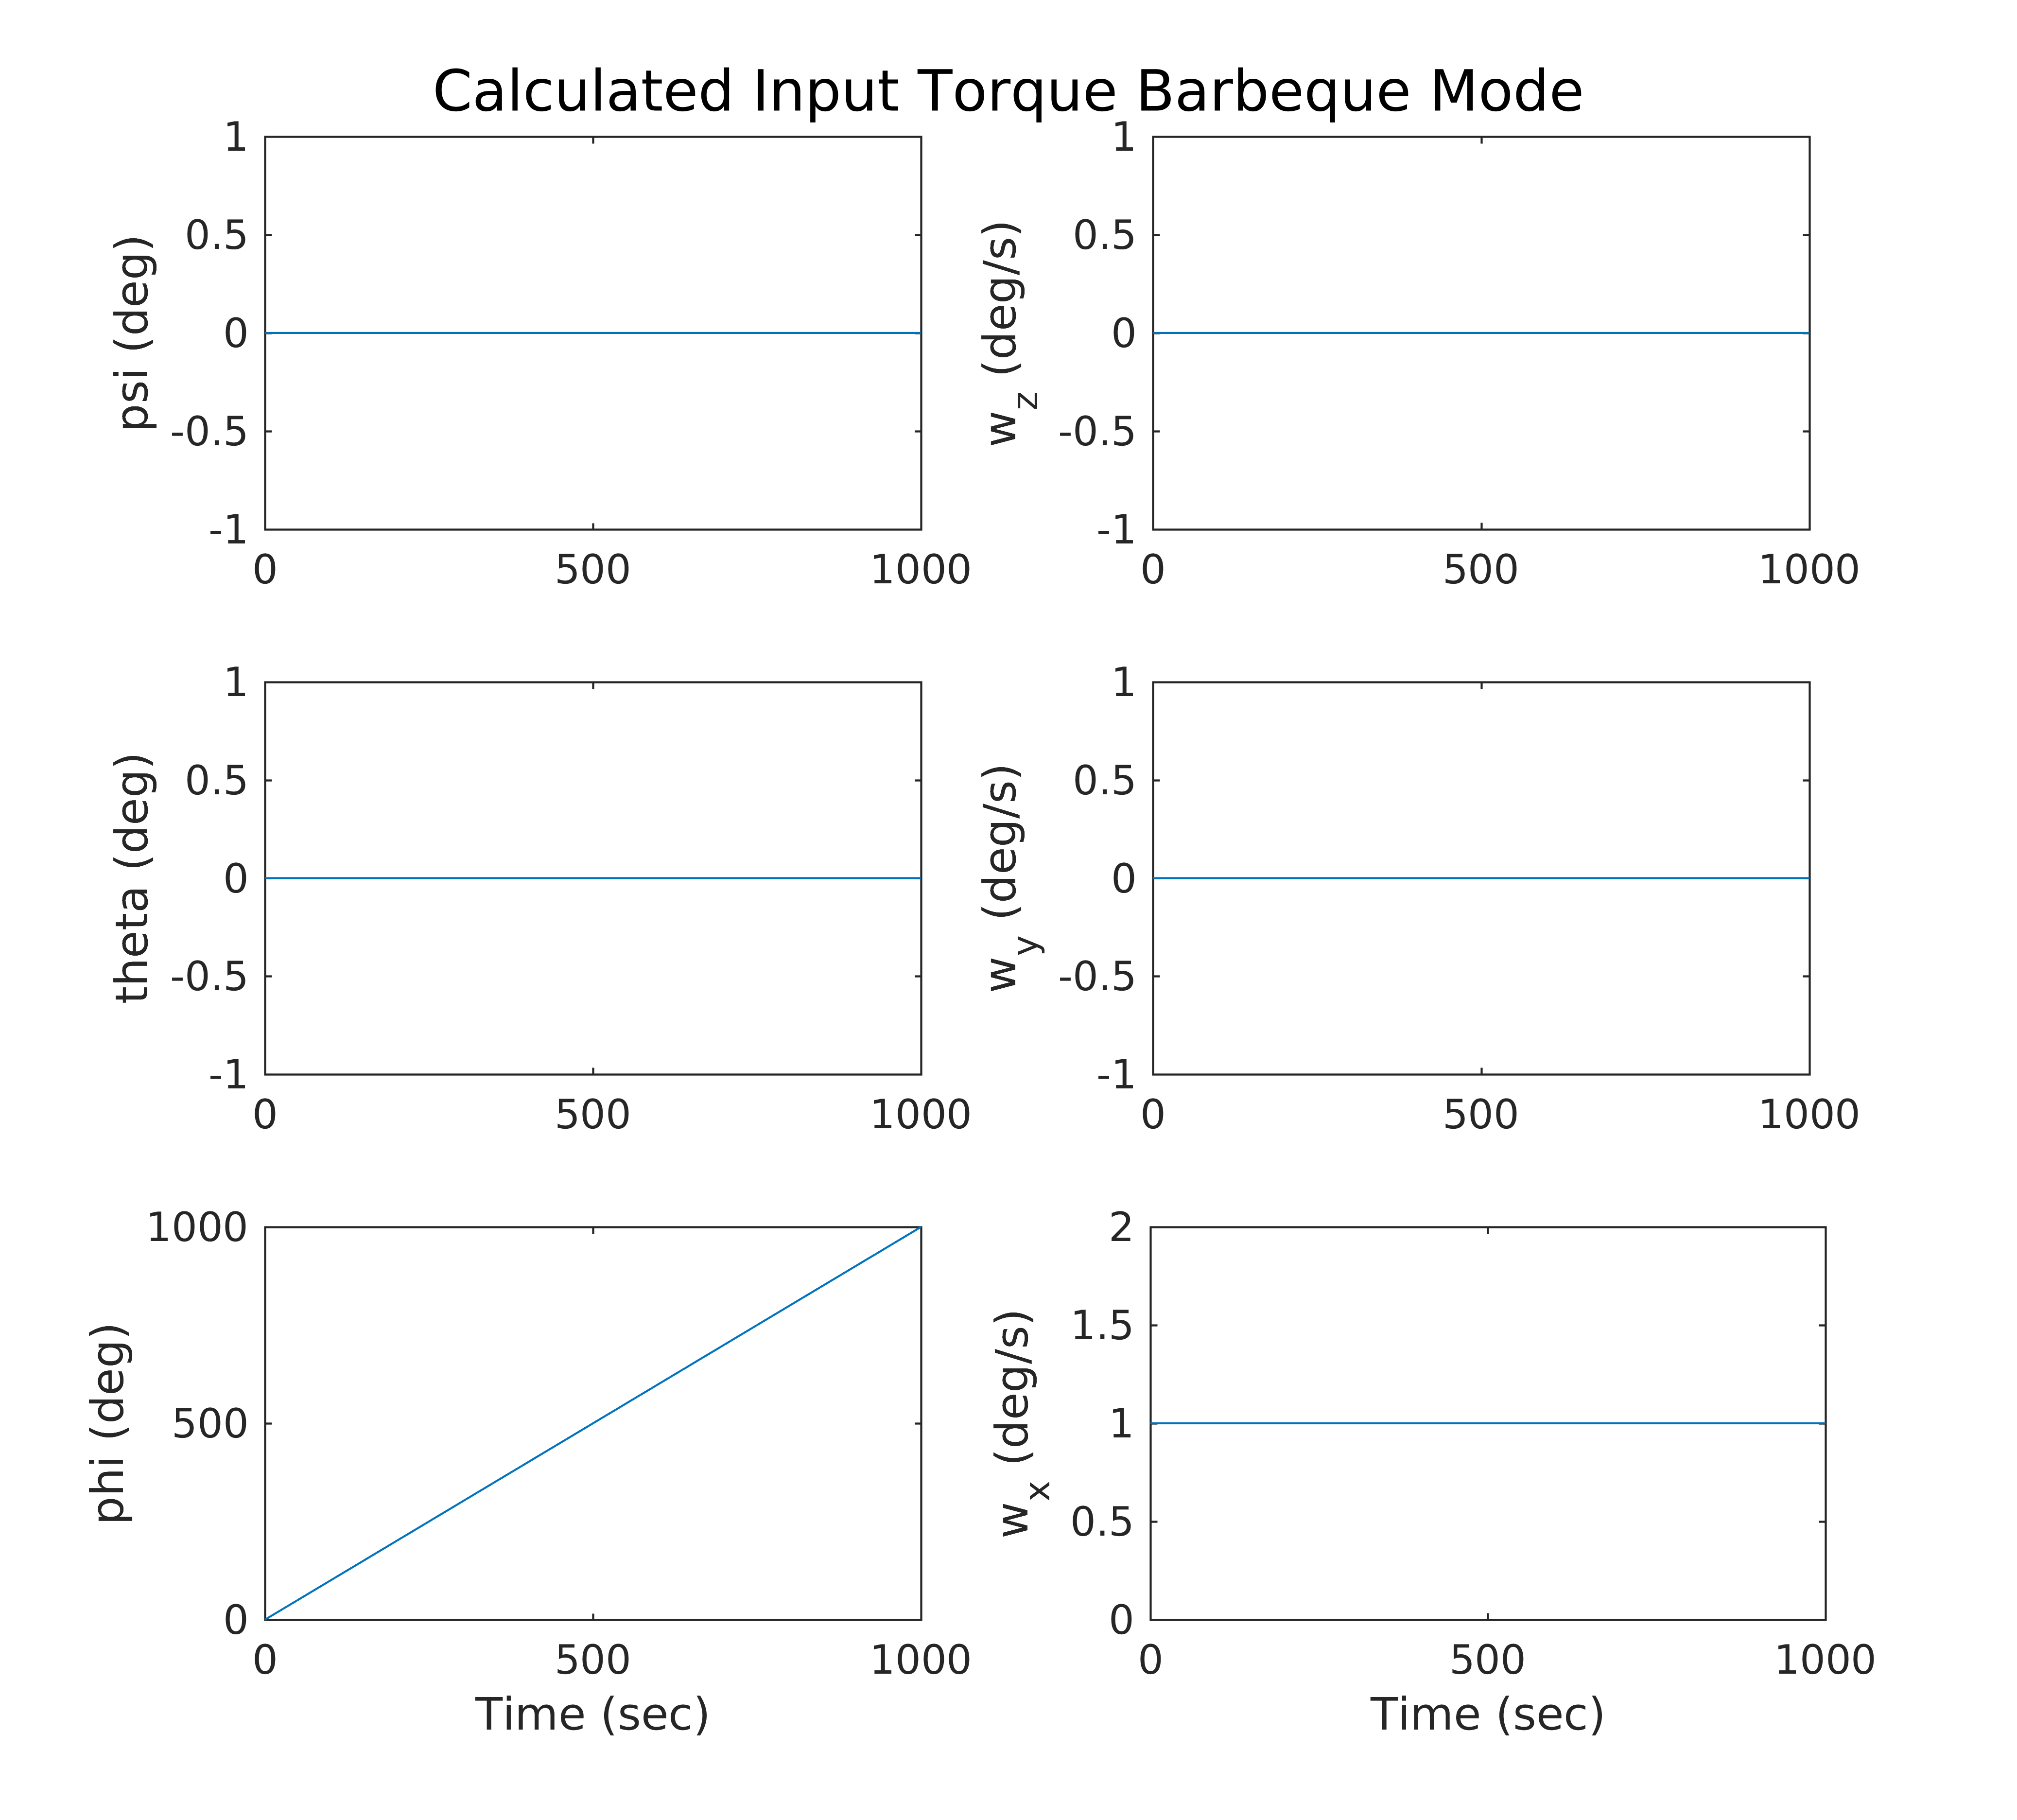
\includegraphics[width=\linewidth]{calc_torque_bbq_mode.png}
  \caption{This figure contains the simulated response to the calculated torque inputs for barbeque mode.}
  \label{fig:calc_torque}
\end{figure}

\begin{figure}[H]
  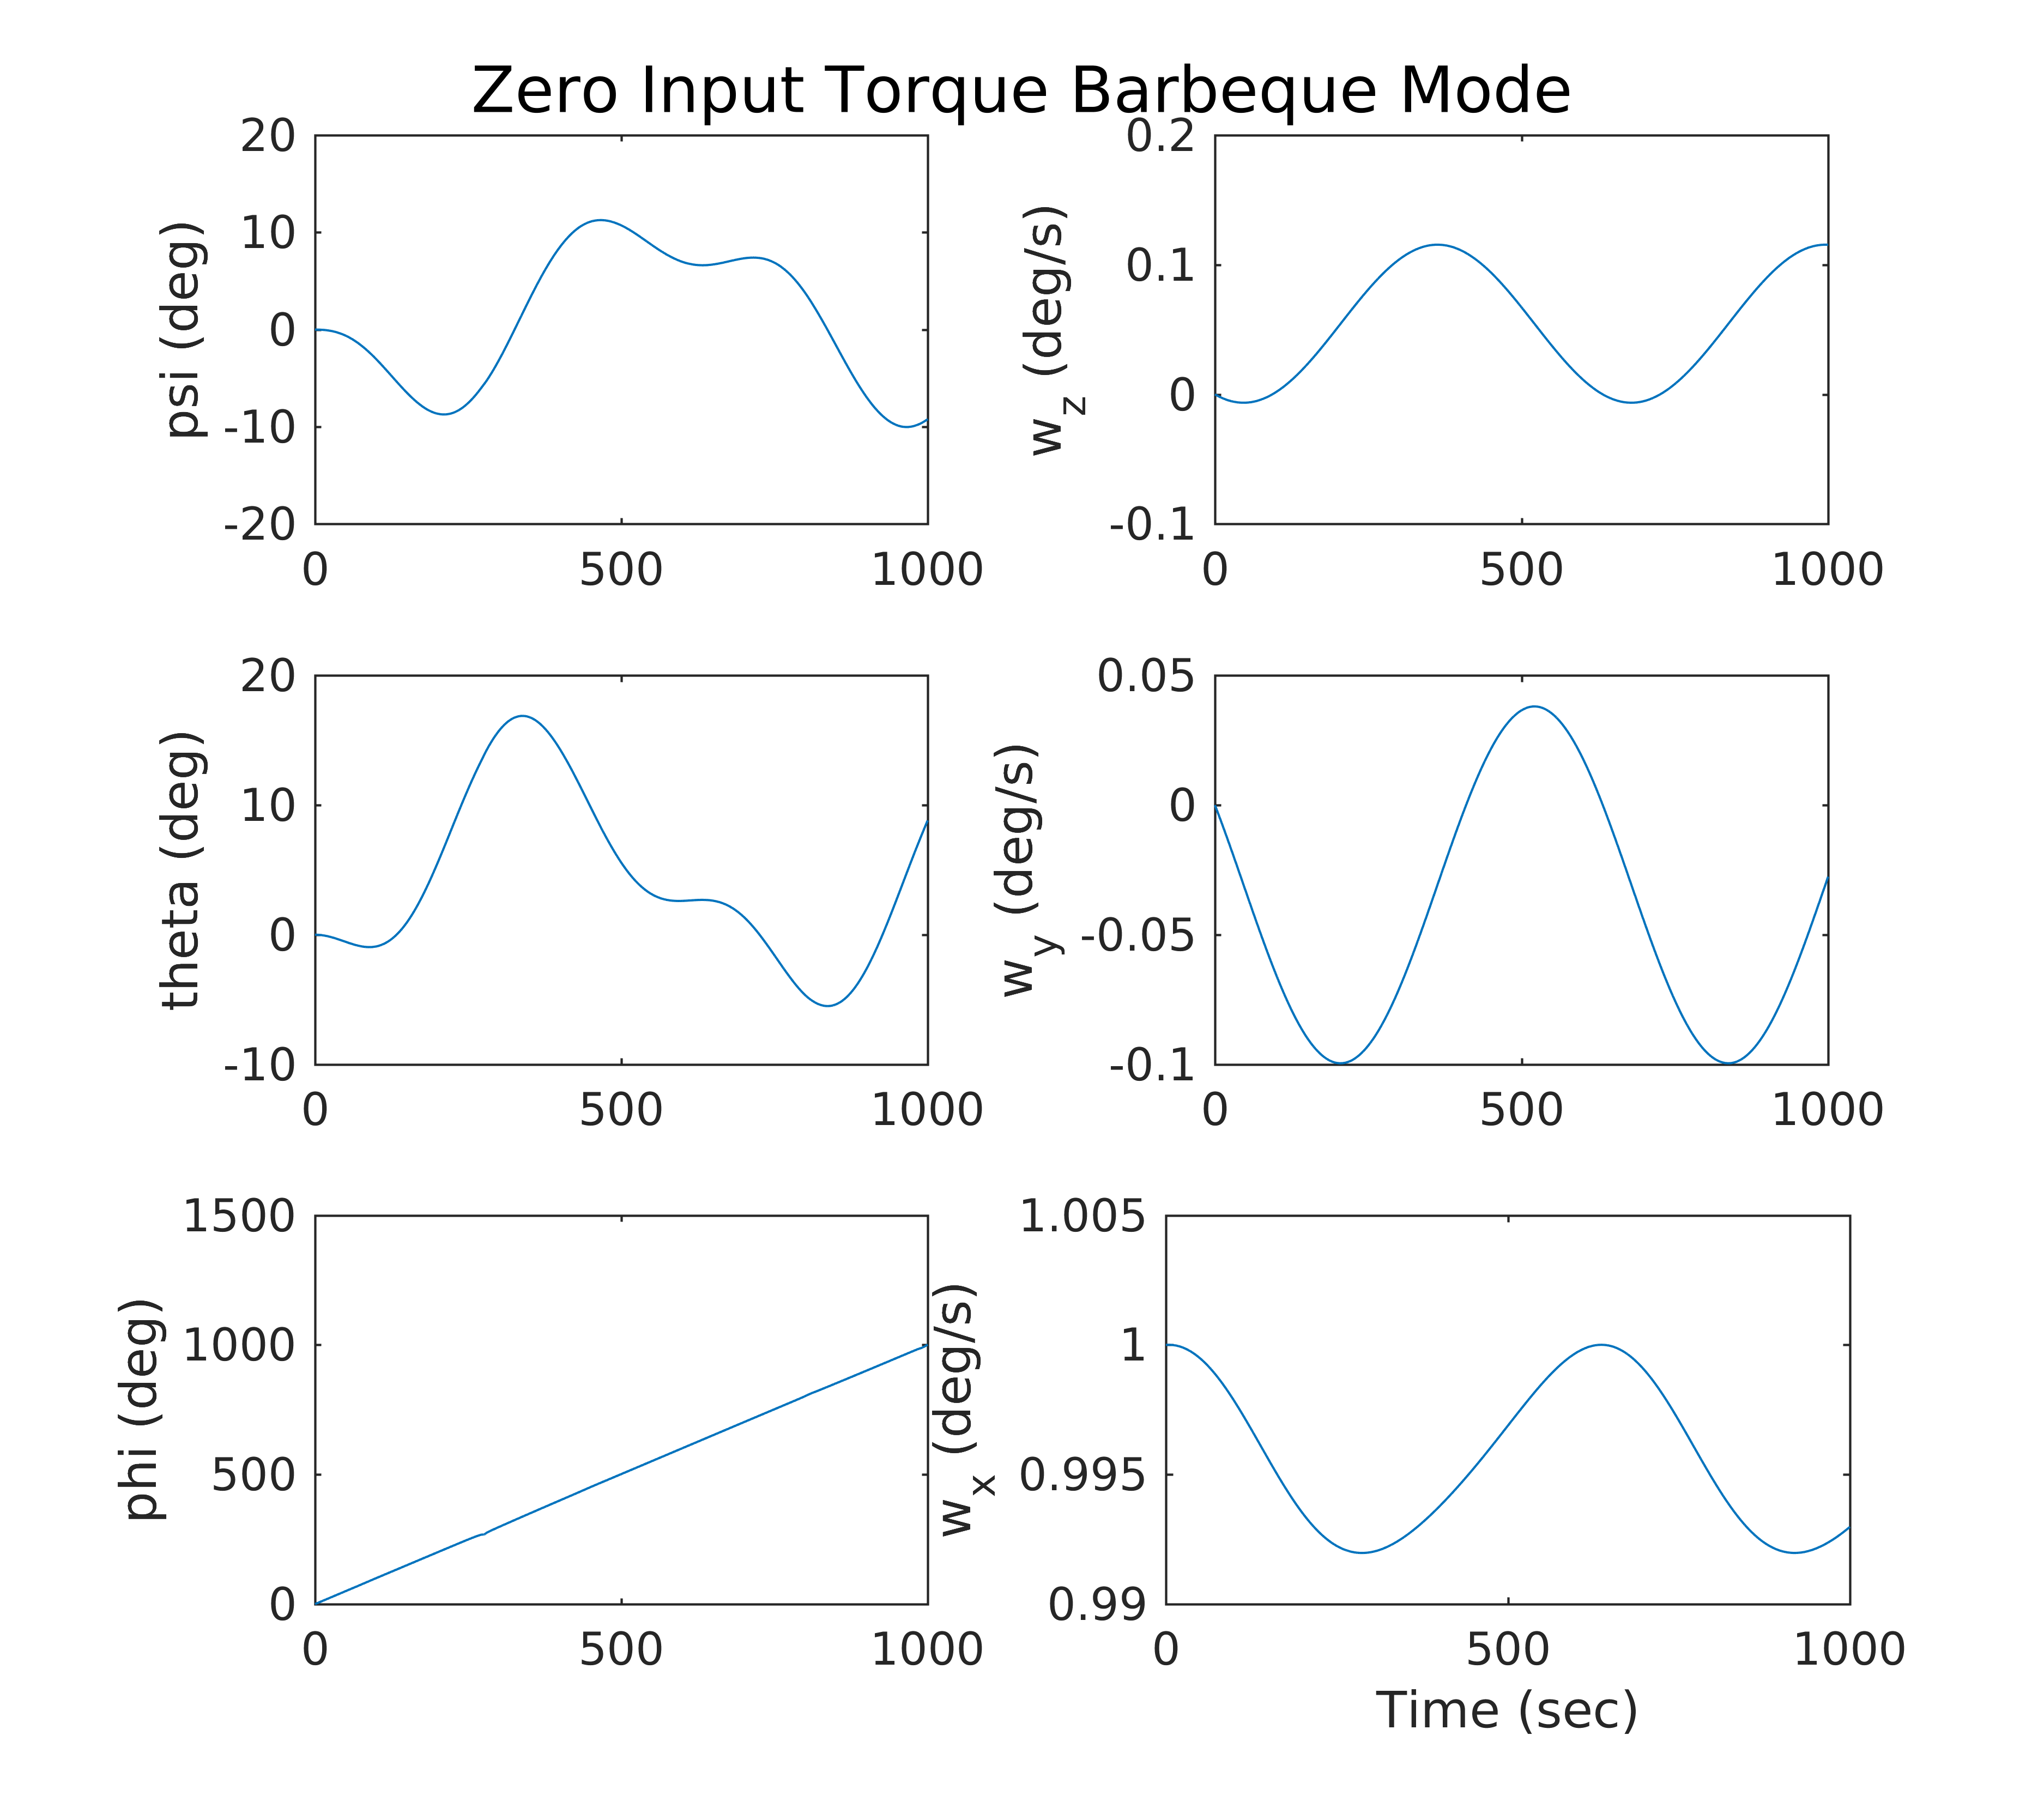
\includegraphics[width=\linewidth]{zero_torque_bbq_mode.png}
  \caption{This figure contains the simulated response to zero torque inputs in barbeque mode.}
  \label{fig:zero_torque}
\end{figure}

\section{Task D: Control Moment Gyroscope Model}
\subsection{Part (a): Mathematical Model}
While the CSM didn't actually use Control Moment Gyroscopes (CMGs) to provide torques, we used them to create a model for how to apply torques to achieve desired motion of the CSM. A CMG was placed on each axis of the B frame, and given the same rotor  angular velocity $\Omega$. We also assumed that $\Omega >> \dot{\theta} >> \omega$, which allowed us to simplify our calculations without losing too much model fidelity. Using these assumptions and differentiating the equation for angular momentum, $\mathbf{H} = I \mathbf{\omega}$, we arrived at Eqs. \ref{CMGMx} - \ref{CMGMz}. $I_r$ is the Inertia of each CMG rotor about its axis of rotation, $\dot{\theta}$ is the rate of change of CMG gimbal angle. 

\begin{equation}\label{CMGMx}
    M_x = I_r\Omega \dot{\theta_1} sin{\theta_1} - I_r\Omega \dot{\theta_3} cos{\theta_3} \:\text{N-m}
\end{equation}

\begin{equation}\label{CMGMy}
    M_y = I_r\Omega \dot{\theta_2} sin{\theta_2} - I_r\Omega \dot{\theta_1} cos{\theta_1} \:\text{N-m}
\end{equation}

\begin{equation}\label{CMGMz}
    M_z = I_r\Omega \dot{\theta_3} sin{\theta_3} - I_r\Omega \dot{\theta_2} cos{\theta_2} \:\text{N-m}
\end{equation}

\subsection{Part (b): Rotor Inertia Calculation}
To calculate the applied torques, we needed to determine a value for $I_r$ so that we could apply Eqs. \ref{CMGMx} - \ref{CMGMz} in our equations of motion. We assumed that each CMG can achieve $\dot{\theta}_{max} = \ 30 \ deg/s$, and that the CSM desired accelerations did not exceed $\dot{\omega}_x = 5 \ deg/s^2$ and $\dot{\omega}_y = \dot{\omega}_z = 2.5 \ deg/s^2$. 

Assuming that the CSM starts from rest and zero orientation, we were able to use Eqs. \ref{CMGMx} - \ref{CMGMz} along with the Euler equations for single-axis rotation to determine a minimum rotor inertia of $\mathbf{I_r = 11.9038}$ \:\textbf{kg-}$\mathbf{m^2}$.

\section{Task E: More Simluations and Calculations}
\subsection{Part (a): Matlab Function}
We created and submitted a matlab function called \verb|mielke_kraus_cmg.m| that simulates the general case rotational motion of the CSM in response to applied torques from the CMGs.


\subsection{Part (b): Simluated Response to Simple Applied CMG Gimbal Angles}
We simulated and plotted the response to the CMG gimbal angle inputs shown in Eqs.~\ref{eq:th1} - \ref{eq:th3} (see Figure~\ref{fig:taske_b}).
\begin{equation}\label{eq:th1}
    \theta_1(t) = 15 sin(\dfrac{2 \pi}{30} t) \:\text{deg}
\end{equation}
\begin{equation}\label{eq:th2}
    \theta_2(t) = 0 \:\text{deg}
\end{equation}
\begin{equation}\label{eq:th3}
    \theta_3(t) = 0 \:\text{deg}
\end{equation}

Table~\ref{tab:max_min} on page~\pageref{tab:max_min} includes the maximum and minimum values for both the general case and simplified case.

\begin{figure}[H]
  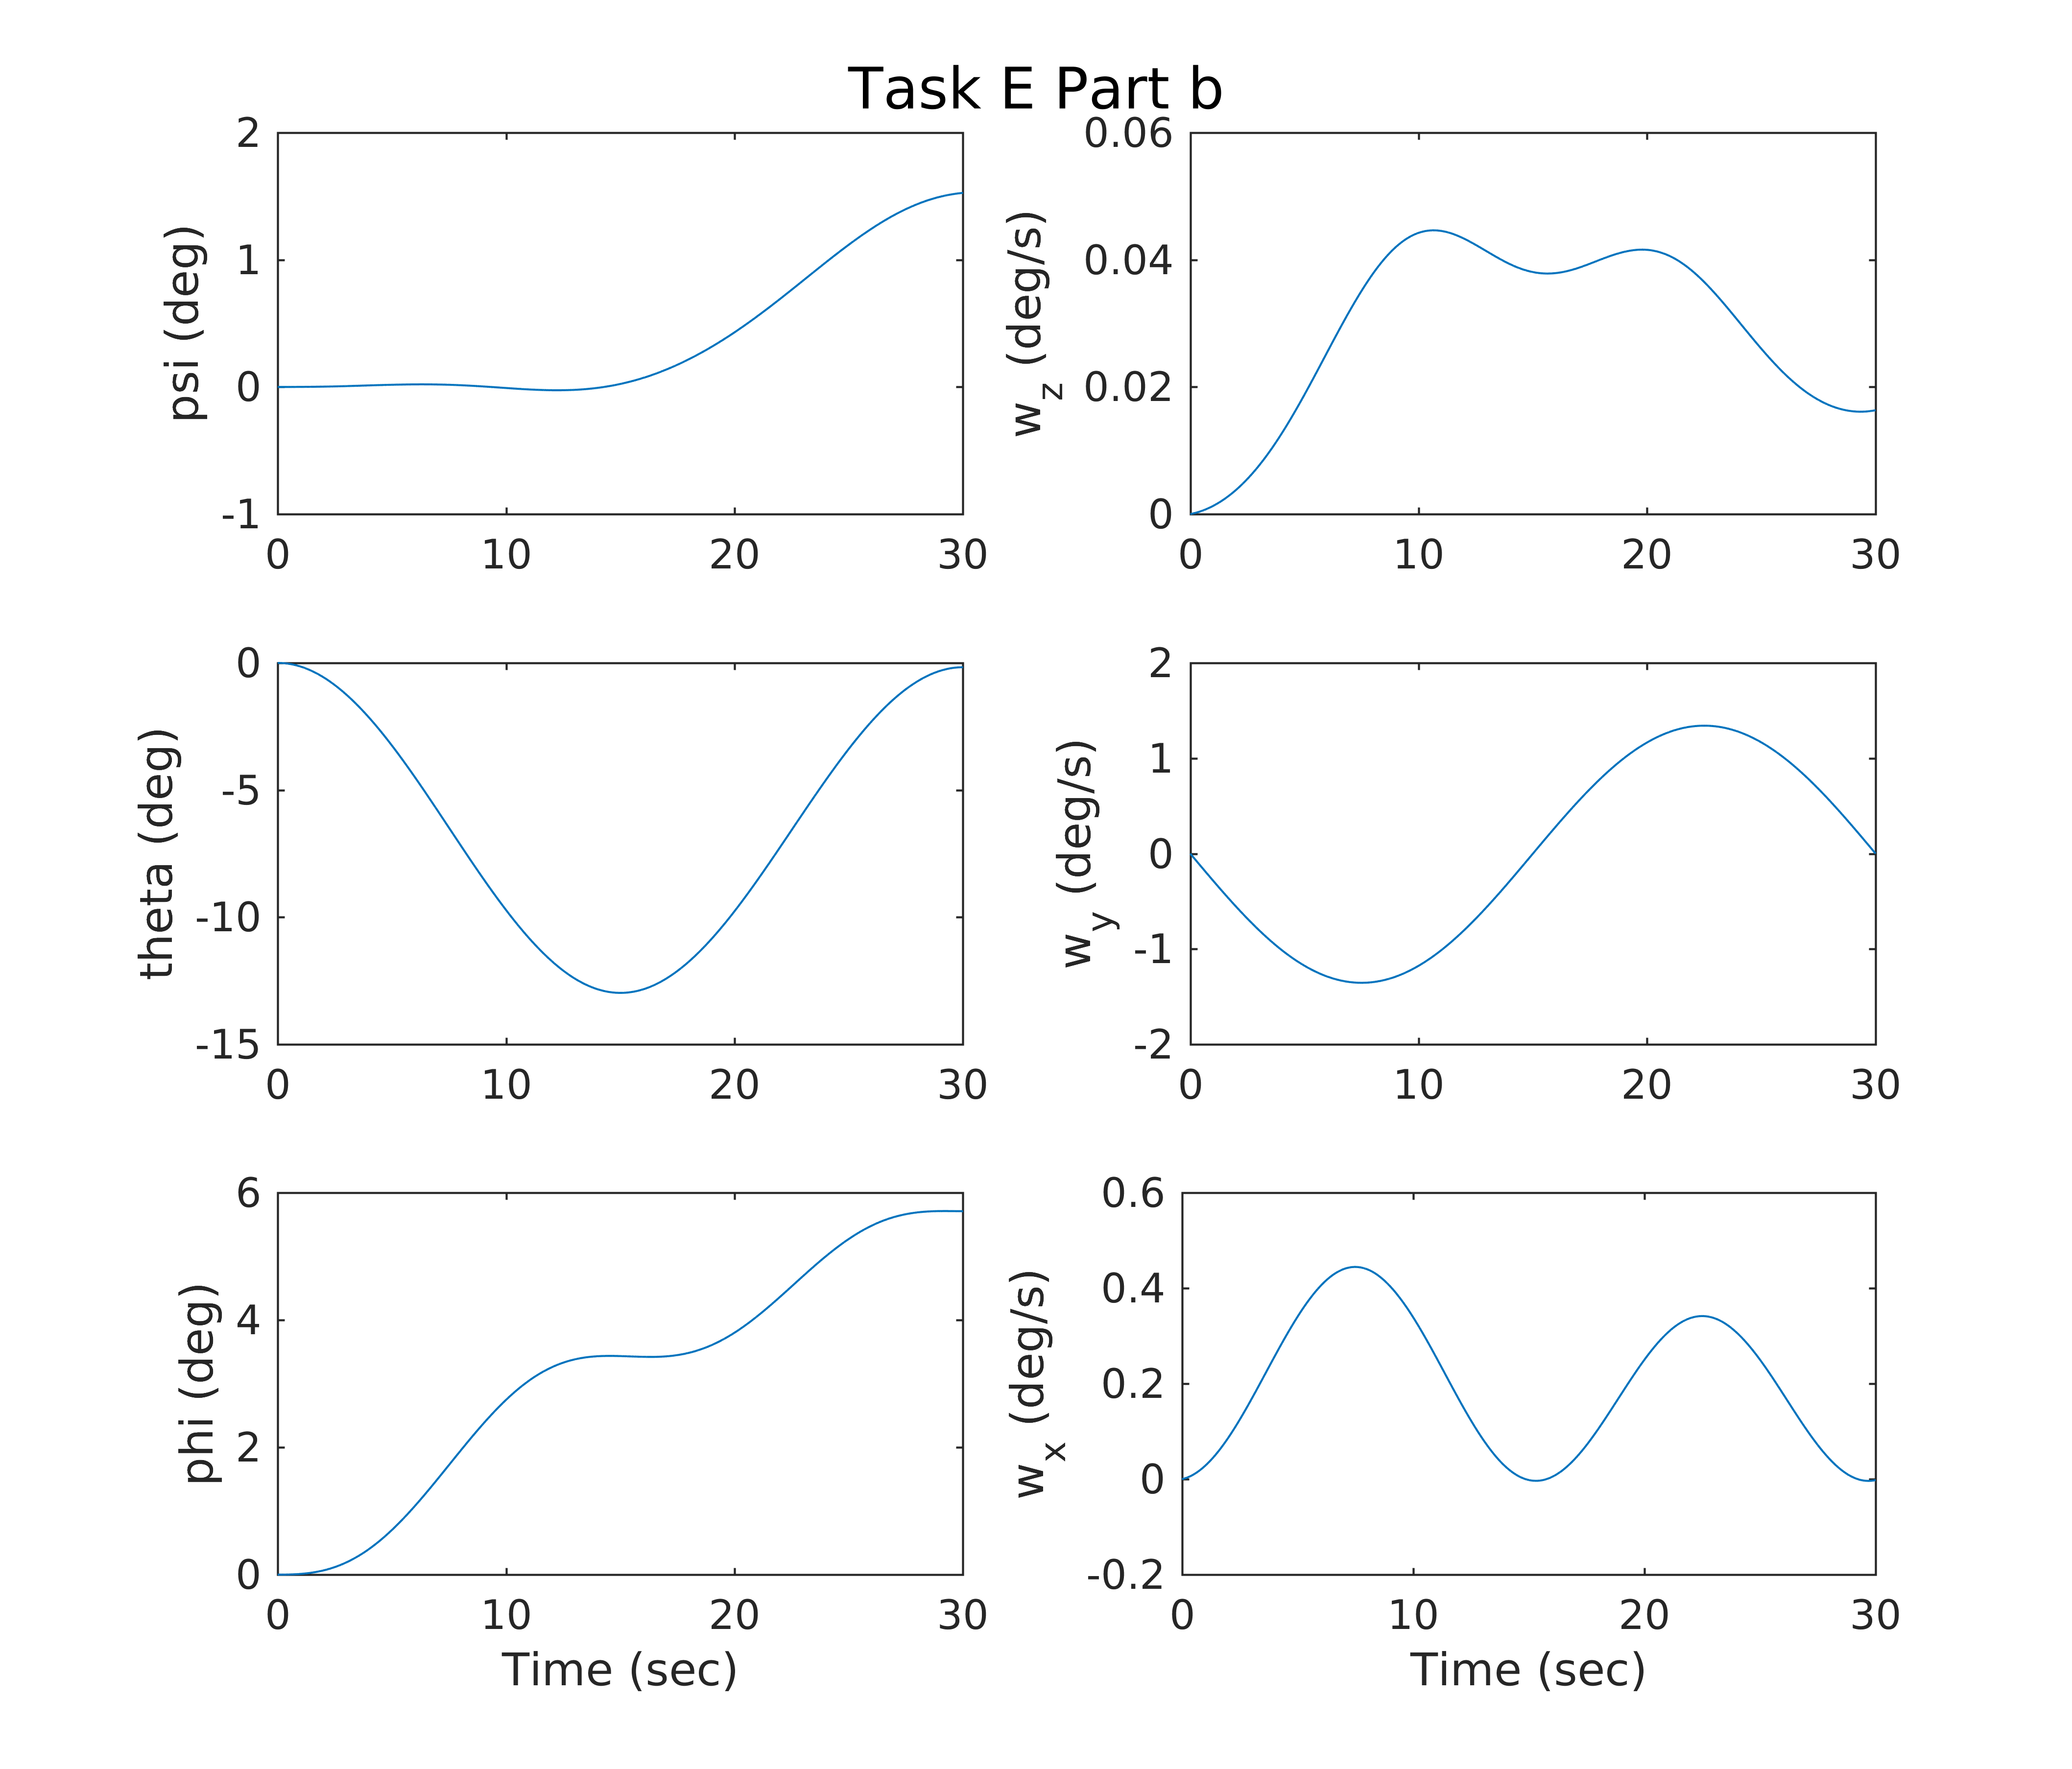
\includegraphics[width=\linewidth]{task_e_part_b.png}
  \caption{This figure contains the general case simulated response to the CMG angles in Eqs.~\ref{eq:th1} - \ref{eq:th3}.}
  \label{fig:taske_b}
\end{figure}

In response to the questions given in the handout, we can explain the behavior of the motion by using the equations of motion for the simplified case, or when there are no products of inertia. Using these equations, we can see that if we vary $\theta_1$, this affects the $M_x$ moment, which causes an acceleration $\alpha_x$ and angular velocities $\omega_y$ and $\omega_z$. Also, $M_y$ is affected, which causes acceleration $\alpha_y$ and angular velocities $\omega_x$ and $\omega_z$. 

Initially, the angle $\theta_1$ is 0, with all $\omega$ values zero as well. From Eqs. \ref{CMGMx} and \ref{CMGMy}, we can determine that at the beginning of the motion, there should be a negative acceleration in $\omega_y$ and zero acceleration in the other directions, which we can see is the case. We also note that as time increases, $\omega_x$ will begin to increase as the moment in x increases, which is also seen. Due to using the General Case for our simulation, we also see a minor contribution to $\omega_z$ as the CSM goes through its motions.

Since the moments are not too large, the CSM stays near its starting angles, and we can approximate how they should be moving by the behavior of the angular velocities
The euler angles seen make sense, as initially we see a negative $\theta$ and a zero $\psi$ and $\phi$. As time increases, $\phi$ begins to increase, as we would expect, and eventually we get minor contributions to $\psi$. 

\subsection{Part (c): Simulated Response to Applied CMG Gimbal Angles}
We simulated and plotted the response to the CMG gimbal angle inputs shown in Eqs.~\ref{eq:th1c} - \ref{eq:th3c} (see Figure~\ref{fig:taske_c}).
\begin{equation}\label{eq:th1c}
    \theta_1(t) = 15 (\dfrac{1}{1 + e^{-0.3 t}} - 0.5) \:\text{deg}
\end{equation}
\begin{equation}\label{eq:th2c}
    \theta_2(t) = 5 sin(\dfrac{2 \pi}{30} t) \:\text{deg}
\end{equation}
\begin{equation}\label{eq:th3c}
    \theta_3(t) = -5 sin(\dfrac{2 \pi}{30} t) \:\text{deg}
\end{equation}

Table~\ref{tab:max_min} on page~\pageref{tab:max_min} includes the maximum and minimum values for the general case.

\begin{figure}[H]
  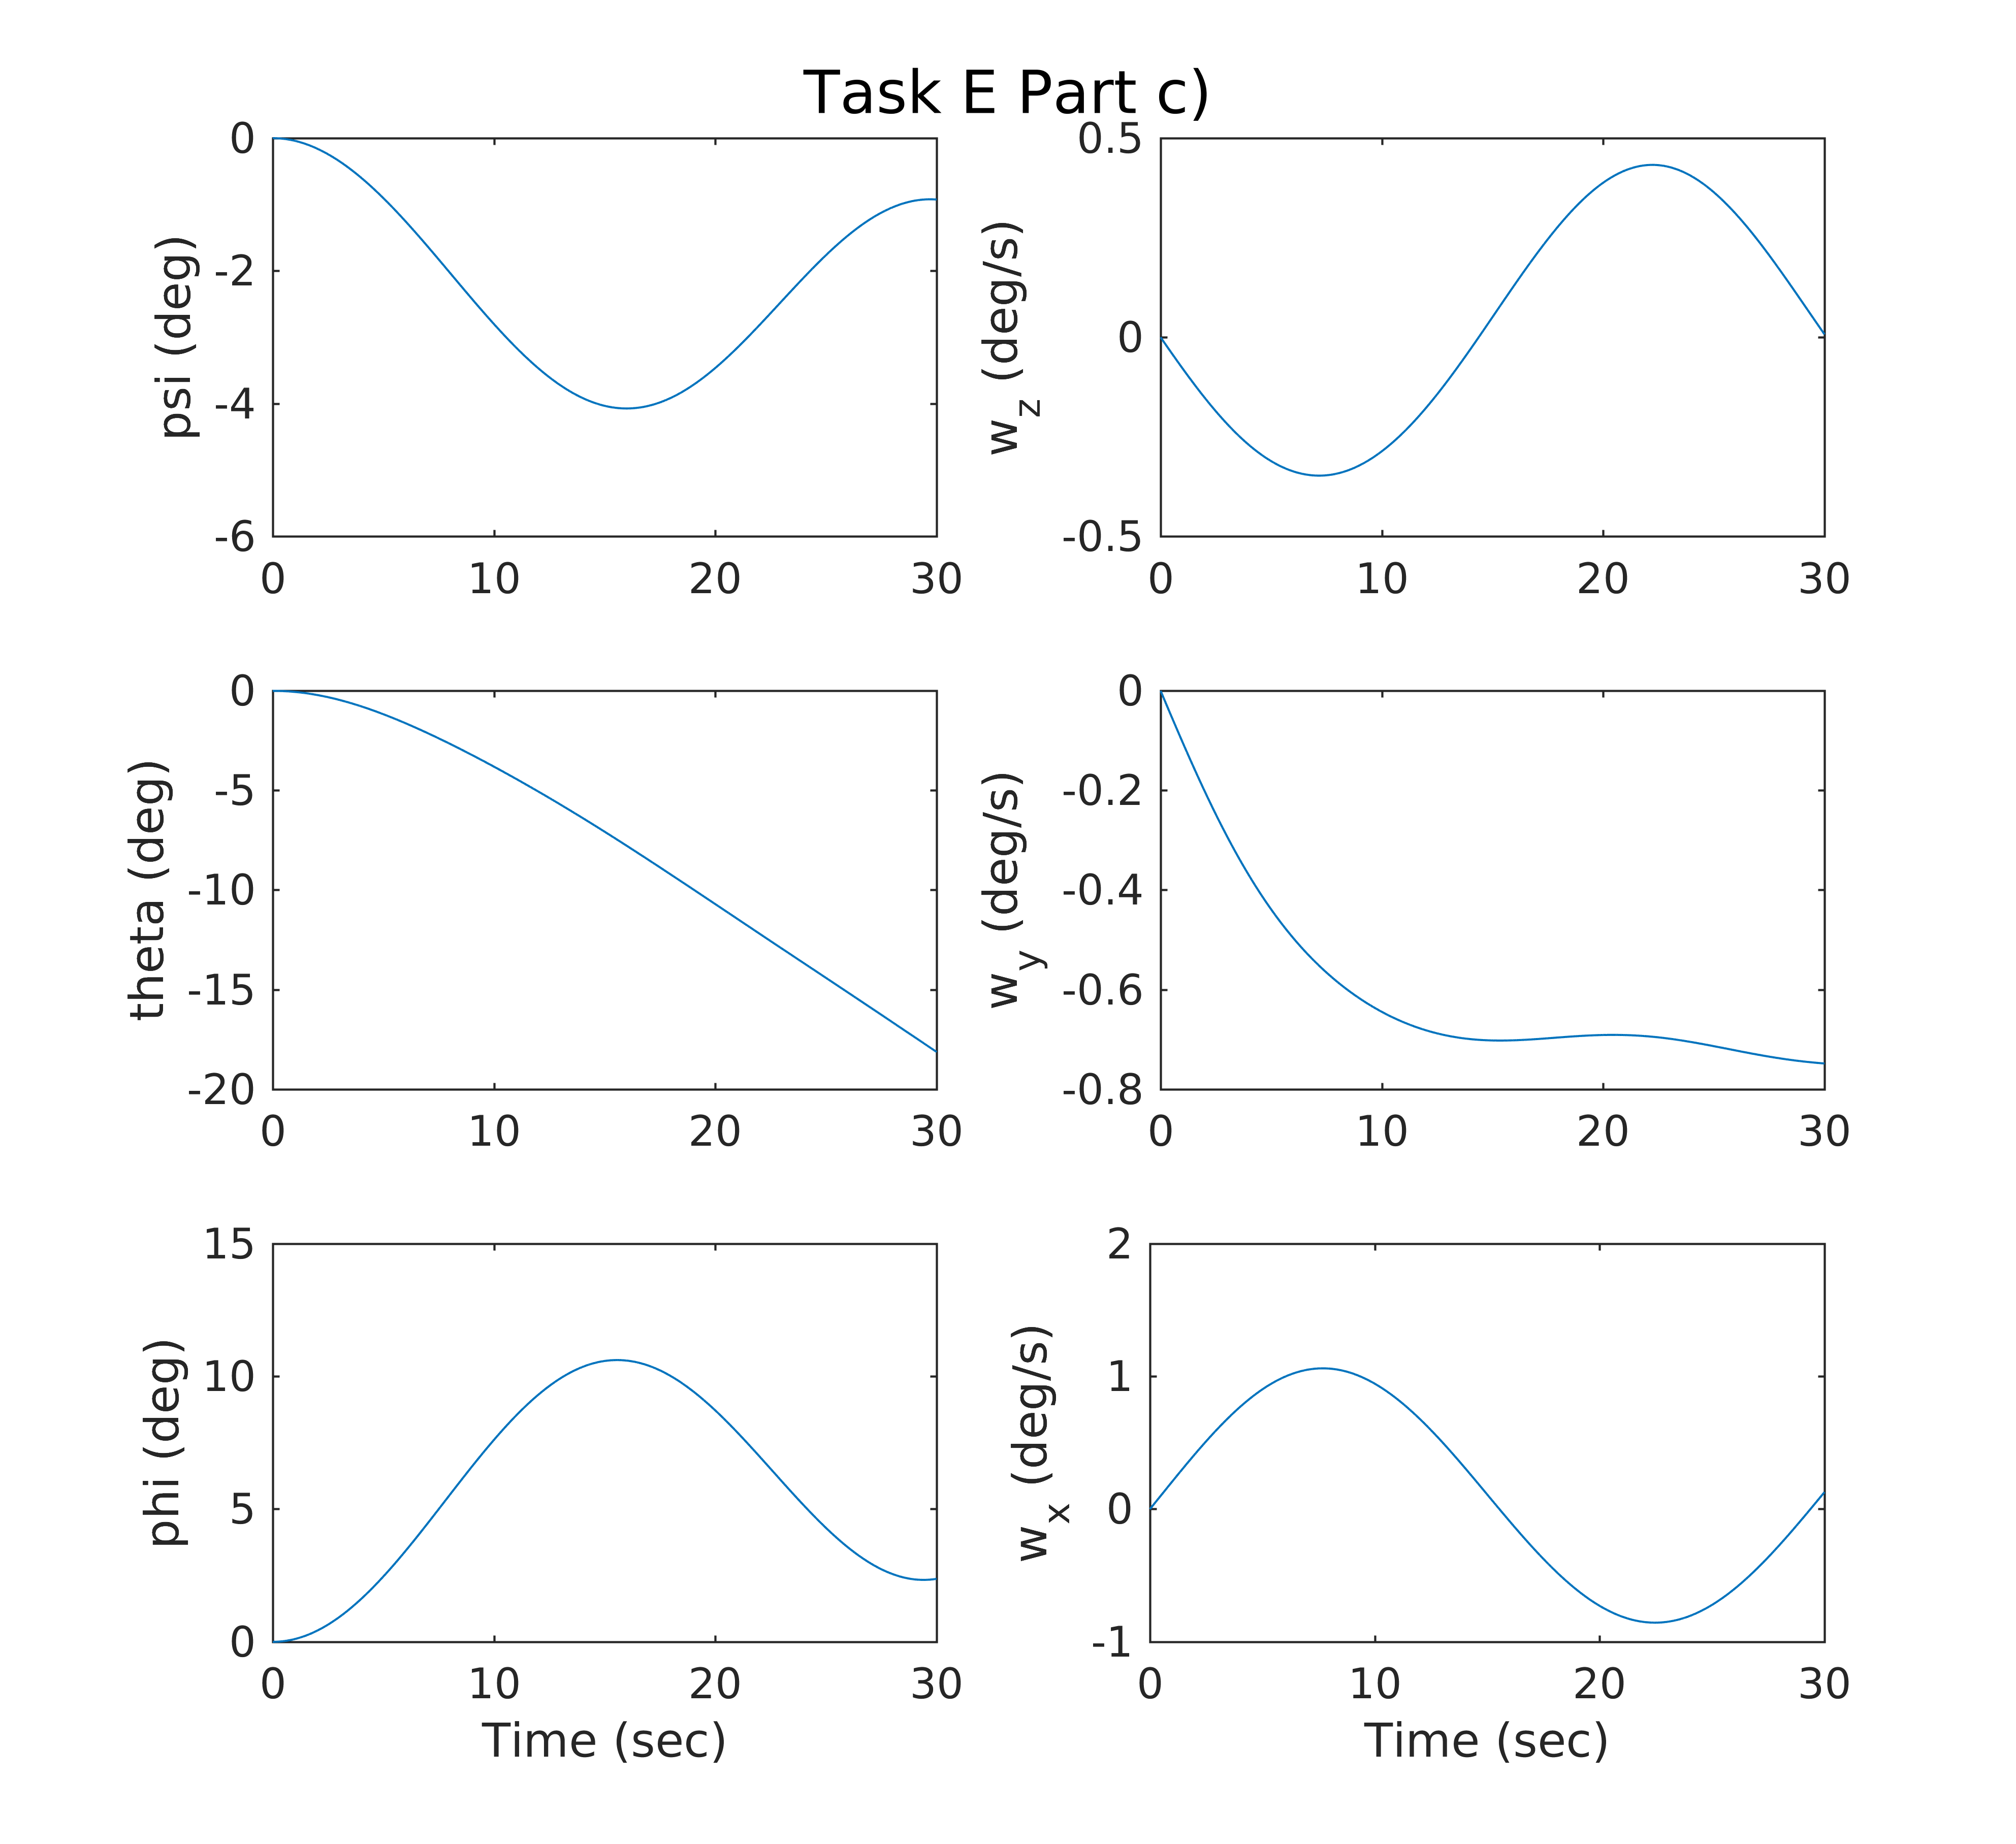
\includegraphics[width=\linewidth]{task_e_part_c.png}
  \caption{This figure contains the simulated response to the CMG angles in Eqs.~\ref{eq:th1c} - \ref{eq:th3c}.}
  \label{fig:taske_c}
\end{figure}

\begin{table}[H]
\centering
\begin{tabular}{c|c|c|c|c|c|c}
 \multicolumn{7}{c}{Task C Part b: General Case: Applied Torques} \\
 \hline
 & $\omega_x$ & $\omega_y$ & $\omega_z$ & $\psi$ & $\theta$ & $\phi$ \\
 \hline
 Min & -1.2698 & 0 & -0.049952 & 0 &  0 & 0\\
 \hline 
 Max & 1.2544 & 1.0431 & 0.40755 & 7.2497 & 15.213 & 12.633 \\
 \hline
 \multicolumn{7}{c}{Task C Part b: Simplified Case: Applied Torques} \\
 \hline
 & $\omega_x$ & $\omega_y$ & $\omega_z$ & $\psi$ & $\theta$ & $\phi$ \\
 \hline
 Min & -1.2504 & 0 & -0.013363 & 0 & 0 & 0\\
 \hline 
 Max & 1.2448 & 1.0464 &  0.42209 & 7.3428 & 15.332 & 12.564 \\
 \hline
 \multicolumn{7}{c}{CMG Task E Part b) General Case} \\
 \hline
 & $\omega_x$ & $\omega_y$ & $\omega_z$ & $\psi$ & $\theta$ & $\phi$ \\
 \hline
 Min & -0.0036583 & -1.3544 & 0 & -0.025904 & -12.975 & 0\\
 \hline 
 Max & 0.44452 & 1.3421 & 0.04464 & 1.5266 & 0 & 5.7117 \\
 \hline
 \multicolumn{7}{c}{CMG Task E Part b) Simplified Case} \\
 \hline
 & $\omega_x$ & $\omega_y$ & $\omega_z$ & $\psi$ & $\theta$ & $\phi$ \\
 \hline
 Min & -0.000259 & -1.3488 & -.0000189 & -0.14382 & -12.93 & 0\\
 \hline 
 Max & 0.39641 & 1.35 & 0.03015 & 1.1148 & 0 & 5.8318 \\
 \hline
 \multicolumn{7}{c}{CMG Task E Part c) General Case} \\
 \hline
 & $\omega_x$ & $\omega_y$ & $\omega_z$ & $\psi$ & $\theta$ & $\phi$ \\
 \hline
 Min & -0.85564 & -0.74846 & -0.3473 & -4.072 & -18.133 & 0\\
 \hline 
 Max & 1.06 & 0 & 0.43292 & 0 & 0 & 10.612 \\
 \hline
\end{tabular}
 \caption{\label{tab:max_min}This table includes the maximum and minimum values for the various simulations. All units are in degrees for the Euler angles and degrees/second for the angular velocities about the x, y, and z axes.}
\end{table}

\section{Task F: Animated Simluation of CSM Motion}
For this portion of the project, we decided to create an animated simulator of the CSM motion in response to torque inputs. The animator takes in a time vector and euler angle vectors that have been calculated by solving the equations of motion (see Task E or Task C). These angles are used to create the motion of the CSM in Matlab. The CSM drawings are comprised of the cone shape of the CM and the cylinder shape of the SM, as well as the body fixed axes attached to the CSM. A sample motion is shown in Fig. \ref{fig:csmmotion}, where the inputs are those used for Barbque mode (see Section. \ref{BBQ}). The gray cylinder and cone are the CSM, the blue axis is the x-axis, the green axis is the y-axis, and the red axis is the z-axis. As we can see, the CSM object is rotating about its x-axis, as is expected for the Barbeque mode.

Our function is called \verb|animate_CSM|(t, $\phi$, $\theta$, $\psi$, n). The variables t, $\phi$, $\theta$, and $\psi$ are column vectors of the time and the respective euler angles (in degrees). The variable n is the playback speed. For example, if t went from 0 to 30 seconds, and if n was set to 1, the animation would take approximately 30 seconds. If n was set to 10, the animation would take approximately 3 seconds. 

\begin{figure}[H]
  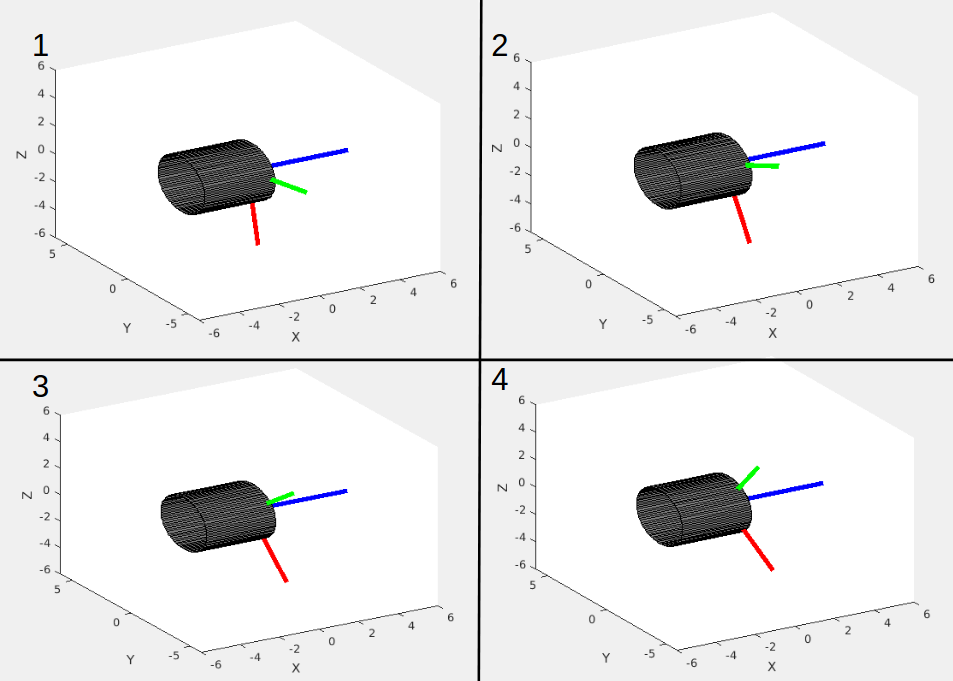
\includegraphics[width=\linewidth]{CSMmotion.png}
  \caption{Screenshots of animation of CSM in response to Barbeque mode inputs.}
  \label{fig:csmmotion}
\end{figure}

\end{document}

